\chapter{Latome Hardware Design}\label{ch:latome-firmware}
% \parskip4pt \parindent12pt

\section{Specifications}\label{sec:specifications}
\subsection{The Liquid Argon Calorimeter Data Path}\label{sec:lar}
The LAr Calorimeter is made of 180,000 cells which are then summed up to form 34,048 supercells. The 12-bit readings of 8 supercells are serialized into one packet and sent through one optic fiber. The 116 LATOME boards are each connected to 48 optic fibers, thus receiving data from \(48\times8=384\) supercells. These boards are responsible for transforming the ADC levels into energy levels, reorganizing the data and summing some energies for LATOMEs covering specific regions of the detector and distributing the data to the Feature Extraction (FEX) system. The FEX system is responsible for processing the data and sending it to the Level 1 Trigger system.
% TODO: Precise what kind of cells

The FEX system is made of 3 groups: the Global Feature Extractor (gFEX), the Jet Feature Extractor (jFEX) and the Electron Feature Extractor (eFEX). Within these groups, gFEX only contains one board which gets summed data from all LATOMEs, thus showing the lowest granularity but with one board covering the whole detector. Then the jFEX is made of 6 boards, each receiving data from 19 LATOMEs, and finally the eFEX, with the highest granularity, is made of 24 boards, each receiving data from 4 LATOMEs.

\subsection{The LATOME Specifications}\label{sec:latome-specifications}
The part of the LATOME firmware responsible for the conversion of ADC levels into energy levels is referred to as \textit{User Code} in the LAr group. This code is not owned by the LATOME HLS team. However, the team is responsible for the different data organization steps, also called mapping or remapping, and the summing of energies for LATOMEs in specific regions of the detector. Additionally, since the output energies are only encoded on 10 bits, it is necessary to compress the data from 12 to 10 bits via a Multi Linear Encoder (MLE).

Initially, the whole LATOME firmware was written in VHDL. The implementation of all the functionalities took over 8 years and still had timing violations. Because in the next runs of the LHC, the amount of energy and collision is expected to increase, the LATOME design should be optimized to leave space for other functionalities, and sustain the increase in data.

\section{Current LATOME Firmware}\label{sec:existing-design}

The original design is characterized by more clock domain crossings than the current one.

\begin{figure}
    \centering
    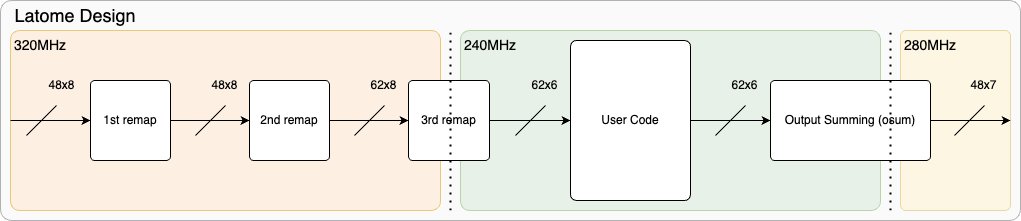
\includegraphics[width=1\textwidth]{latome_fw_vhdl.png}
    \caption{Original VHDL Design}
    \label{fig:original-vhdl-design}
\end{figure}

Because bunch crossings (BC) happen at a frequency of 40MHz, it is necessary to run the different blocks of the design at multiples of this frequency. The figure\ref{fig:original-vhdl-design} shows three different frequencies being used. At the first remap stage, since the frames are made of 8 words, it is necessary to run the blocks at 320MHz. Then the frames become 6 words long, corresponding to a frequency of 240MHz. Finally, the FEX systems expect 7 32 bits words, thus the frequency is 280MHz.

\begin{figure}[htb]
    \centering
    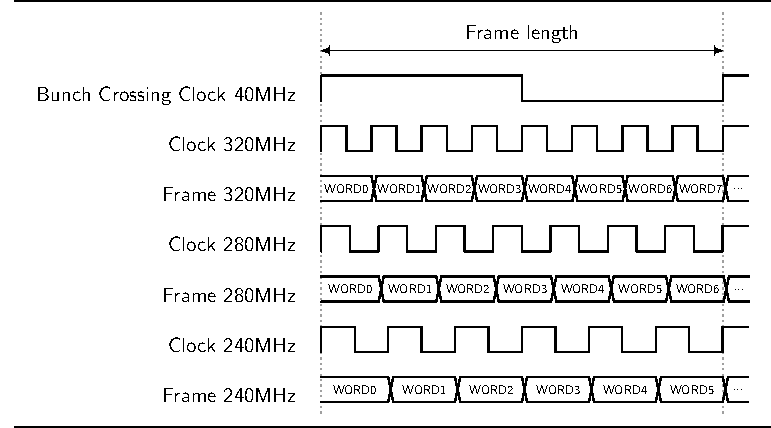
\includegraphics{timings/bc_clocks}
    \caption{Different clocks used in the design}
    \label{fig:bc-clocks}
\end{figure}

These clock domain crossings made the original implementation very complex...
%TODO: add more about the complexity of the original design

\section{Leveraging Time vs Space Division Multiplexing}\label{sec:leveraging-time-division-multiplexing}

When a chunk of data is available at a given time for processing, it can all be processed at the same time, or pieces after pieces.
Processing simultaneously all the data offers the advantage of a reduced latency, but requires creating copies of the processing 
blocks for each piece. A sequential processing gives the possibility of having just one processing block treating the data step 
by step at a price of latency.

\subsection{Time Division Multiplexing}\label{sec:time-division-multiplexing}
The time division multiplexing approach consists in sharing the resources, or processing blocks, by routing each piece of data depending on time \(t\). Choosing this implementation can be intuitive as computers usually process data using frames of 32 to 64 bits. It has the advantage of reusing design blocks hence possibly reducing area usage, but performs poorly in case of data dependencies. If the word from time \(t=0\) of the frame needs to be available at the same time as the one of \(t=4\), the logic becomes very complex thus canceling the positive area impact unlocked by resource sharing.

This sequential processing approach requires counters used by multiplexers to latch the input data at the right moments. This approach is represented in figure \ref{fig:time-division-multiplexing}.

\begin{figure}
    \begin{subfigure}[c]{.5\textwidth}
        \centering
        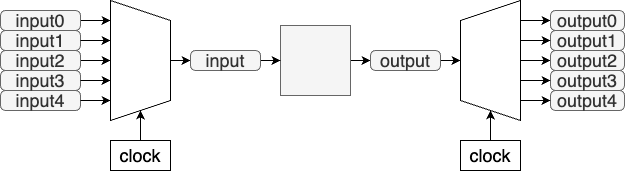
\includegraphics[width=1\linewidth]{tdm.png}
        \caption{Block Diagram}
    \end{subfigure}
    \begin{subfigure}[c]{.5\textwidth}
        \centering
        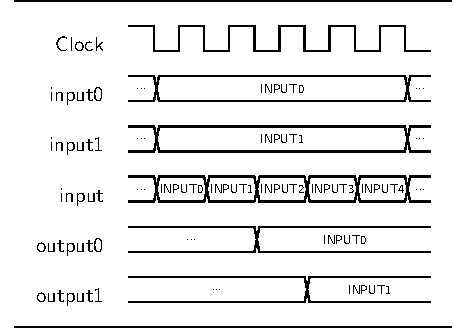
\includegraphics[width=1\linewidth]{../timings/tdm.pdf}
        \caption{Timing}
    \end{subfigure}
    \caption{Time Division Multiplexing}
    \label{fig:time-division-multiplexing}
\end{figure}

\subsection{Space Division Multiplexing}
Another way of treating the data is to make it all available at the same time, as parallel inputs of the processing block. This approach is more natural as it is closer to what humans experience; we see, hear, feel, taste at the same time, not one after the other. It is represented in figure \ref{fig:space-division-multiplexing}. Space Division Multiplexing generally offers small latencies, as every block runs in parallel and reduces the use of sequential logic which would be required in TDM. In fact, using a parallel logic, some processing blocks can become purely combinational ones.

\begin{figure}
    \begin{subfigure}{.5\textwidth}
        \centering
        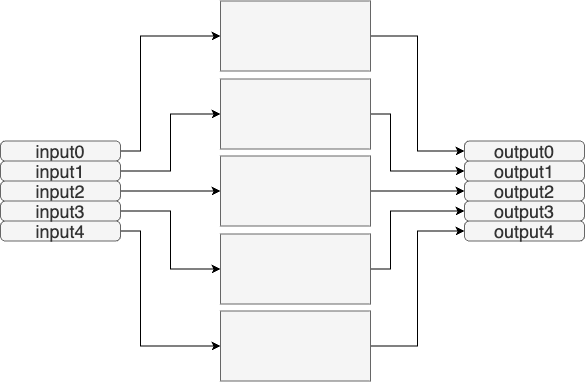
\includegraphics[width=1\linewidth]{sdm.png}
        \caption{Block Diagram}
    \end{subfigure}
    \begin{subfigure}{.5\textwidth}
        \centering
        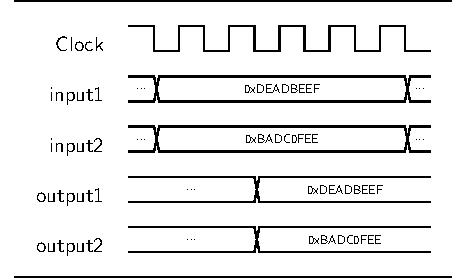
\includegraphics[width=1\linewidth]{../timings/sdm.pdf}
        \caption{Timing}
    \end{subfigure}
    \caption{Space Division Multiplexing}
    \label{fig:space-division-multiplexing}
\end{figure}

\subsection{Tradeoffs}\label{sec:space-versus-time-division-multiplexing}
Whether one approach is better than the other is impossible to determine prior to having a deep understanding of the data processing blocks.
The most common tradeoff is the one of latency at the price of area. But the Maximal Operating Frequency (\(F_{max}\)) can also be traded to 
improve other metrics.

Having access to all variables at the same time makes the code development easier.

\section{New HLS Design}\label{sec:current-hls-design}
When developing the new firmware from the specifications in HLS, very interesting insights from Dr. Marcos Oliveira emphasizing benefits of space division multiplexing were taken into account. By using parallel full frames, the frequency of the design blocks is not locked anymore depending on the frame size. This allows to reduce the logic dedicated only to synchronization and time-division multiplexing which can become very complex when there are dependencies between the words of the frame.

\begin{figure}
    \centering
    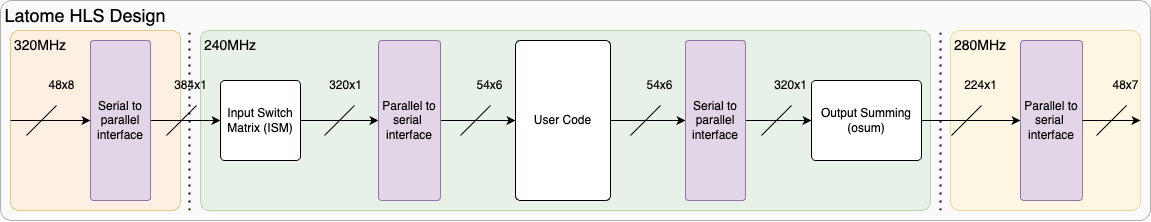
\includegraphics[width=1\textwidth]{latome_fw_hls.png}
    \caption{Current HLS Design}
    \label{fig:current-HLS-design}
\end{figure}

The figure \ref{fig:current-HLS-design} shows that all the remapping and processing blocks except for the User Code are being processed using parallel data. This is possible thanks to the serial-to-parallel and parallel-to-serial data transformation blocks. This approach drastically simplifies the design and showed very promising results in terms of area reduction, reduced latency.
% TODO: add more promising results

\begin{figure}
    \centering
    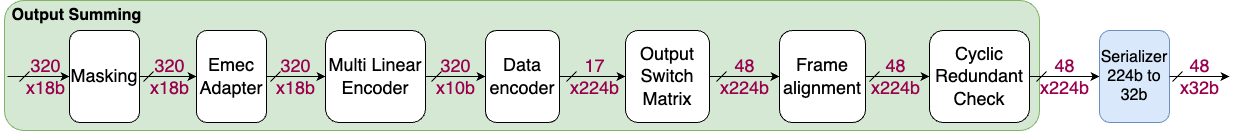
\includegraphics[width=1\textwidth]{osum_v6.png}
    \caption{Output Summing Block Diagram}
    \label{fig:osum-v6}
\end{figure}

The Output Summing was completely redesigned and broken down in different blocks which are represented in figure \ref{fig:osum-v6}. It is made of the following blocks:
\begin{itemize}
    \item Masking: responsible for disabling some inputs depending on the detector region that a specific LATOME treats
    \item Emec Adapter: this block performs additional summing for the LATOME responsible for the EMEC region of the detector
    \item Multi Linear Encoder (MLE): Since the ADC readings are 12 bits long but the FEX systems requires 10 bits long energy levels, this block encodes the ADC readings on 10 bits
    \item Data Encoder: Once the encoded energy levels are ready, this block creates 17 frames of 224 bits representing the whole data
    \item Output Switch Matrix (OSM): This switch matrix routes the 17 224 bits frames to the different FEX systems that the LATOME is connected too
    \item Frame Alignment: Each couple of BC, the LATOME does not send any data but instead it sends an alignment frame built by this block
    \item CRC9: This final block appends to the last 9 bits of each frame a CRC9 value which it computes
\end{itemize}